\section{Background and Motivation}
\label{sec:bg-motivation}

\subsection{MoE Serving and Cross-Layer Prefetching}

\noindent
A Mixture-of-Experts (MoE) layer routes each token through only a small subset of its expert sub-networks~\cite{shazeer2017outrageously, fedus2021switch, yang2024xmoe, chen2022towards, zhou2022mixture}. At inference time, this sparsity reshapes the per-layer cost from being \emph{compute-bound} to being \emph{memory-bound}: per-token FLOPs drop with the activation ratio, but each MoE layer must fetch a different subset of expert weights, and an MoE model's expert footprint typically exceeds the device HBM by an order of magnitude. A serving runtime therefore cannot keep all experts resident; it must \emph{predict} which experts will be activated next and \emph{move} them onto the device ahead of execution.

\smallskip
\noindent
Cross-layer prefetching is the dominant template for hiding these expert transfers. While computing layer~$\ell$, the runtime forecasts the experts likely to be activated in the next~$S$ MoE layers and issues their transfers on a separate stream so that they overlap with the compute of layers~$\ell, \ldots, \ell{+}S{-}1$. We call~$S$ the \emph{prefetch horizon}. ProMoE~\cite{song2024promoe}, ExpertFlow~\cite{he2024expertflow}, and Hobbit~\cite{tang2024hobbit} all instantiate this template; they choose a single value of~$S$ at deployment time and reuse it across all requests. Crucially, $S$ does not change the model's routing semantics---it controls only how far ahead the system speculates.

\smallskip
\noindent
The choice of~$S$ is what determines whether expert transfers stay off the critical path. \autoref{fig:M1} plots latency against~$S$ for three MoE models on NVIDIA A6000 under a 20\,GB HBM cap. Each curve is U-shaped: below the U-minimum, transfers do not finish within the available compute window and the critical path accumulates exposed waiting; above it, speculative residency exceeds HBM capacity, evictions cascade, and cache pollution amplifies subsequent miss latency. The U-minimum sits at a different~$S$ for each model on the same device. Two questions follow: where does the U-minimum sit on a given deployment, and is it stable enough that we can find it offline?

\begin{figure}
    \centering
    {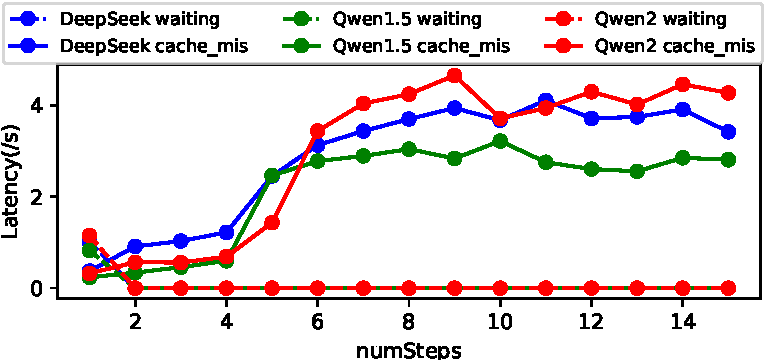
\includegraphics[width=0.99\linewidth]{figures/M1_numstep_latency.pdf}}
    \vspace{-0.5em}
    \caption{Latency vs.\ prefetch horizon~$S$ for three MoE models on
    NVIDIA A6000 under a 20\,GB HBM cap. The y-axis is waiting +
    cache-miss latency (s/request); the x-axis is~$S$ (number of MoE
    layers prefetched ahead). Each curve is U-shaped, and the
    U-minimum sits at a different~$S$ for each model. We show in
    \autoref{sec:bg-motivation:variance} that the minimum also moves
    across devices, batches, and intra-batch token compositions, so
    no offline-tuned~$S$ is robust.}
    \label{fig:M1}
\end{figure}

\subsection{The Optimum Moves Along Three Independent Axes}
\label{sec:bg-motivation:variance}

\noindent
The U-minimum is not stable. Three factors, each independent of the others, shift it. We discuss each in turn and connect it to the failure mode of fixed-horizon systems.

\paragraph{Hardware bandwidth.}
The accelerators used in this work span an order of magnitude in effective host--device bandwidth, from $\sim 8$\,GB/s on AMD RX~6500XT to $\sim 128$\,GB/s on NVIDIA H20 and Ascend~910B. The transfer time of a layer's experts scales inversely with this bandwidth, while the per-layer compute time scales with FLOPs throughput; their ratio determines how many compute-layers' worth of overlap window is available to hide one layer's transfer. On a fast interconnect a small~$S$ already fits transfers inside the overlap window; on a slow one a much larger~$S$ is needed. A fixed-horizon system tuned for one accelerator therefore exposes systematic stalls when migrated to a slower interconnect or a co-tenanted GPU where effective bandwidth has dropped---this is precisely the cross-device brittleness of ProMoE-style runtimes.

\paragraph{Batch scale.}
Even on fixed hardware, the optimal~$S$ shifts with batch size. Larger batches amortize per-layer overhead but also widen the set of concurrently demanded experts and shrink each expert's per-token overlap budget. To make this concrete, let $E_{\text{req}}$ be the experts requested by a batch over the next~$S$ layers, $\hat{E}$ the experts actually prefetched, and $E_{\text{hit}} = E_{\text{req}} \cap \hat{E}$ those that arrive before they are needed. The expert miss ratio is
$
R_{\text{miss}} = 1 - \tfrac{|E_{\text{hit}}|}{|E_{\text{req}}|}.
$
As batch-induced demand diversity grows, $|E_{\text{req}}|$ grows faster than $S$ can keep up, so $R_{\text{miss}}$ rises. \autoref{fig:M3} shows that holding~$S$ fixed and sweeping batch size from 1 to 32 inflates the waiting component of latency by up to $2.5\times$ while the cache-miss component can simultaneously decrease as residency stabilizes. The two components move in opposite directions, so no single~$S$ minimizes both---a fixed-horizon system is forced to trade one for the other.

\begin{figure}
    \centering
    {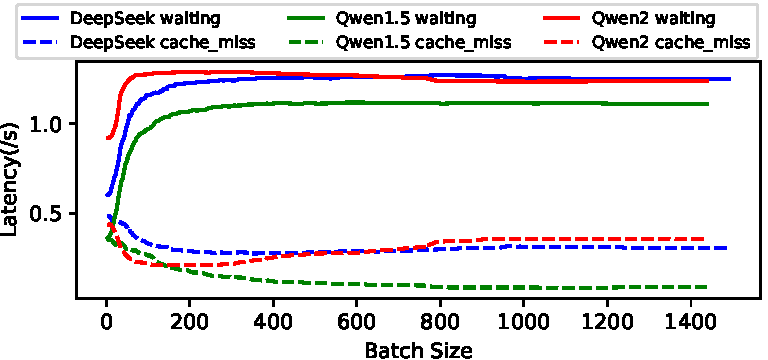
\includegraphics[width=0.99\linewidth]{figures/M3_batchsize_latency.pdf}}
    \vspace{-0.5em}
    \caption{Latency components vs.\ batch size at a fixed~$S$ on
    A6000. The waiting component grows non-monotonically with batch
    size (more concurrent requests $\Rightarrow$ more concurrently
    demanded experts $\Rightarrow$ less per-expert overlap window),
    increasing by up to $2.5\times$, while the cache-miss component
    can decrease as residency stabilizes. The two components move in
    opposite directions, which is precisely why a single offline~$S$
    cannot be optimal across batch sizes.}
    \label{fig:M3}
\end{figure}

\paragraph{Intra-batch token diversity.}
At fixed batch size, requests with different token compositions activate different sets of experts in subsequent layers. We use a lightweight proxy for intra-batch diversity, the sum of pairwise embedding distances:
\[
\text{Dist}(\mathbf{t}) = \sum_{1 \le i < j \le k} \lVert \mathbf{v}_{t_i} - \mathbf{v}_{t_j} \rVert_2,
\]
where $\mathbf{v}_{t_i}$ is the embedding of token $t_i$. \autoref{fig:M5} plots the number of distinct experts activated per layer against batch size and $\text{Dist}(\mathbf{t})$ on three MoE models. At a fixed batch size, requests with high semantic dispersion activate noticeably more experts and exhibit up to $300\%$ end-to-end latency variation compared to low-dispersion requests with the same batch size. A fixed-horizon system that chooses~$S$ on a representative low-dispersion batch therefore systematically under-prefetches on diverse batches, even when the deployment hardware and batch size are unchanged.

\begin{figure}
    \centering
    {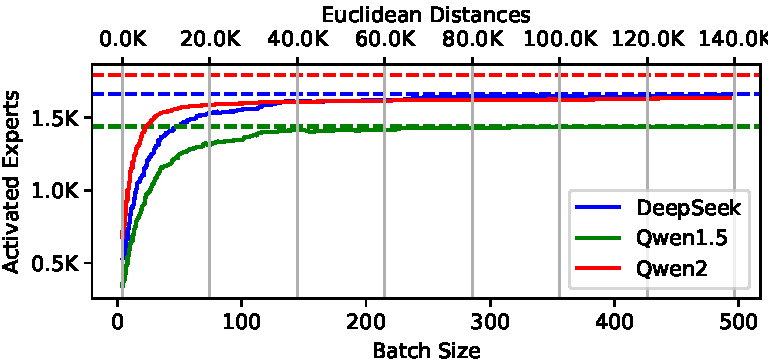
\includegraphics[width=0.99\linewidth]{figures/M5_DeepSeek_Qwen1.5_Qwen2.pdf}}
    \vspace{-0.5em}
    \caption{Number of distinct experts activated per layer vs.\
    batch size (x-axis) and the embedding-dispersion proxy
    $\mathrm{Dist}(\mathbf{t})$ (color), for DeepSeek-V2-Lite,
    Qwen1.5-MoE, and Qwen2-MoE. At fixed batch size, high-dispersion
    requests activate noticeably more experts and incur up to
    $300\%$ latency variation, so dispersion is a useful
    per-request signal for the controller, on top of batch size.}
    \label{fig:M5}
\end{figure}

\subsection{Implications for System Design}
\label{sec:bg-motivation:implications}

\noindent
Putting the three axes together, the U-minimum drifts continuously across (device, workload, request) tuples. For any candidate offline~$S^*$, we can construct a deployment in which some other~$S' \neq S^*$ is strictly better, and we exhibit such cases in our evaluation (\autoref{sec:evaluation}). Tuning~$S$ offline therefore amounts to picking the configuration on which to lose: the engineer chooses one device--workload pair to optimize and accepts a multiplicative latency tax everywhere else. The right object is not a hyperparameter but a control policy that chooses~$S_t$ at each control period in response to current runtime signals. Building such a policy means solving three coupled sub-problems---deriving a stable~$S_t$ from partial, noisy observations of bandwidth, demand, and cache state; predicting which experts will be needed over the next~$S_t$ layers without competing for GPU cycles; and bounding the cost of misprediction so that errors cause at most one DMA, never a cascade of stalls---which we address in \autoref{sec:design:controller}, \autoref{sec:design:forecaster}, and \autoref{sec:design:memory}, respectively.
